\documentclass[a4paper, 10pt, final, garamond]{book}
\usepackage{cours-preambule}

\makeatletter
\renewcommand{\@chapapp}{M\'ecanique -- chapitres}
\renewcommand\thechapter{6 et 7}
\makeatother
\renewcommand{\thefigure}{\arabic{figure}}

% \toggletrue{student}
% \toggletrue{corrige}
% \renewcommand{\mycol}{black}
\renewcommand{\mycol}{gray}

\begin{document}
% \setcounter{chapter}{0}

% \settype{enon}
% \settype{solu_prof}
% \settype{solu_stud}

\chapter{TD~: moment cin\'etique et forces centrales}

% TODO: Recopier corrigé manuel

\section{Gravimètre de \textsc{Holweck-Lejay}}

Une masse ponctuelle $m$ est placée à l'extrémité M d'une tige de masse
négligeable et de longueur $L = \OMr$, articulée en O et mobile dans un plan
vertical. Un ressort «~spirale~» (non représenté sur la figure) exerce sur M,
via la tige, un couple de rappel (notion abordée au chapitre 8) équivalent à un
moment de force dont la projection sur $(\Or z)$ est $\Mc_z = -C\th$ avec $C>0$.

\noindent
\begin{minipage}[]{0.25\linewidth}
	\begin{center}
		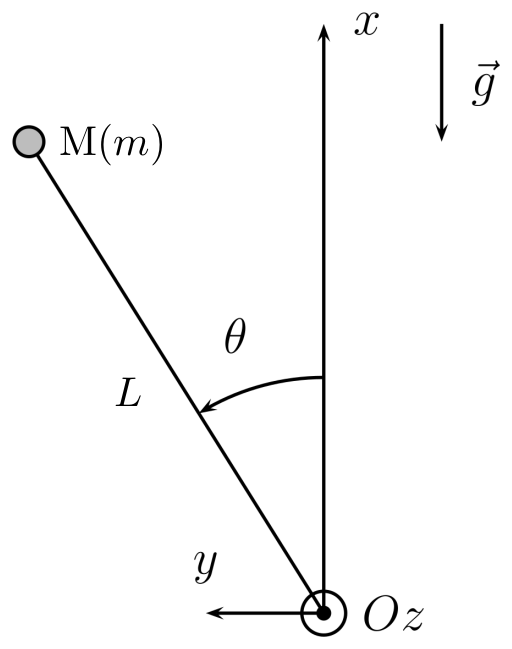
\includegraphics[width=\linewidth]{holweck-plain_m}
	\end{center}
\end{minipage}
\hfill
\begin{minipage}[]{0.70\linewidth}
	\begin{enumerate}
		\item Déterminer, par l'application du théorème du moment cinétique par
		      rapport à l'axe $(\Or z)$, l'équation différentielle vérifiée par
		      $\th$.
		\item À l'aide d'un développement de \textsc{Taylor} autour de $\th =
			      0$, déterminer la condition sur $C$ pour que $\th = 0$ soit une
		      position d'équilibre stable.
		\item Retrouver ce résultat en établissant l'énergie potentielle du
		      ressort spiral puis en étudiant la stabilité par une approche
		      énergétique.
		\item À partir de l'équation différentielle simplifiée à la question 2,
		      calculer la période $T$ des petites oscillations autour de $\th =
			      0$.
		\item En posant $g_0 = C/mL$, déduire des résultats précédents une
		      méthode de mesure de $g$.
	\end{enumerate}
\end{minipage}

\section{Pendule conique}

\noindent
\begin{minipage}{0.70\linewidth}
	Dans un champ uniforme de pesanteur $\gf$ vertical et vers le bas, un point
	matériel M de masse $m$ tourne à la vitesse angulaire $\w$ constante autour
	de l'axe $(\Or z)$, dirigé vers le haut, et décrit ainsi un cercle de centre
	O et de rayon $R$. M est suspendue à un fil inextensible de longueur $L$ et
	de masse négligeable, fixé en un point A de $(\Or z)$. L'angle $\a$ de $(\Or
		z)$ avec AM est constant. \smallbreak On travaille dans le référentiel du
	laboratoire supposé galiléen. On utilisera le repère de la base cylindrique
	tel que $\OM = R\ur$.
\end{minipage}
\begin{minipage}{0.25\linewidth}
	\begin{center}
		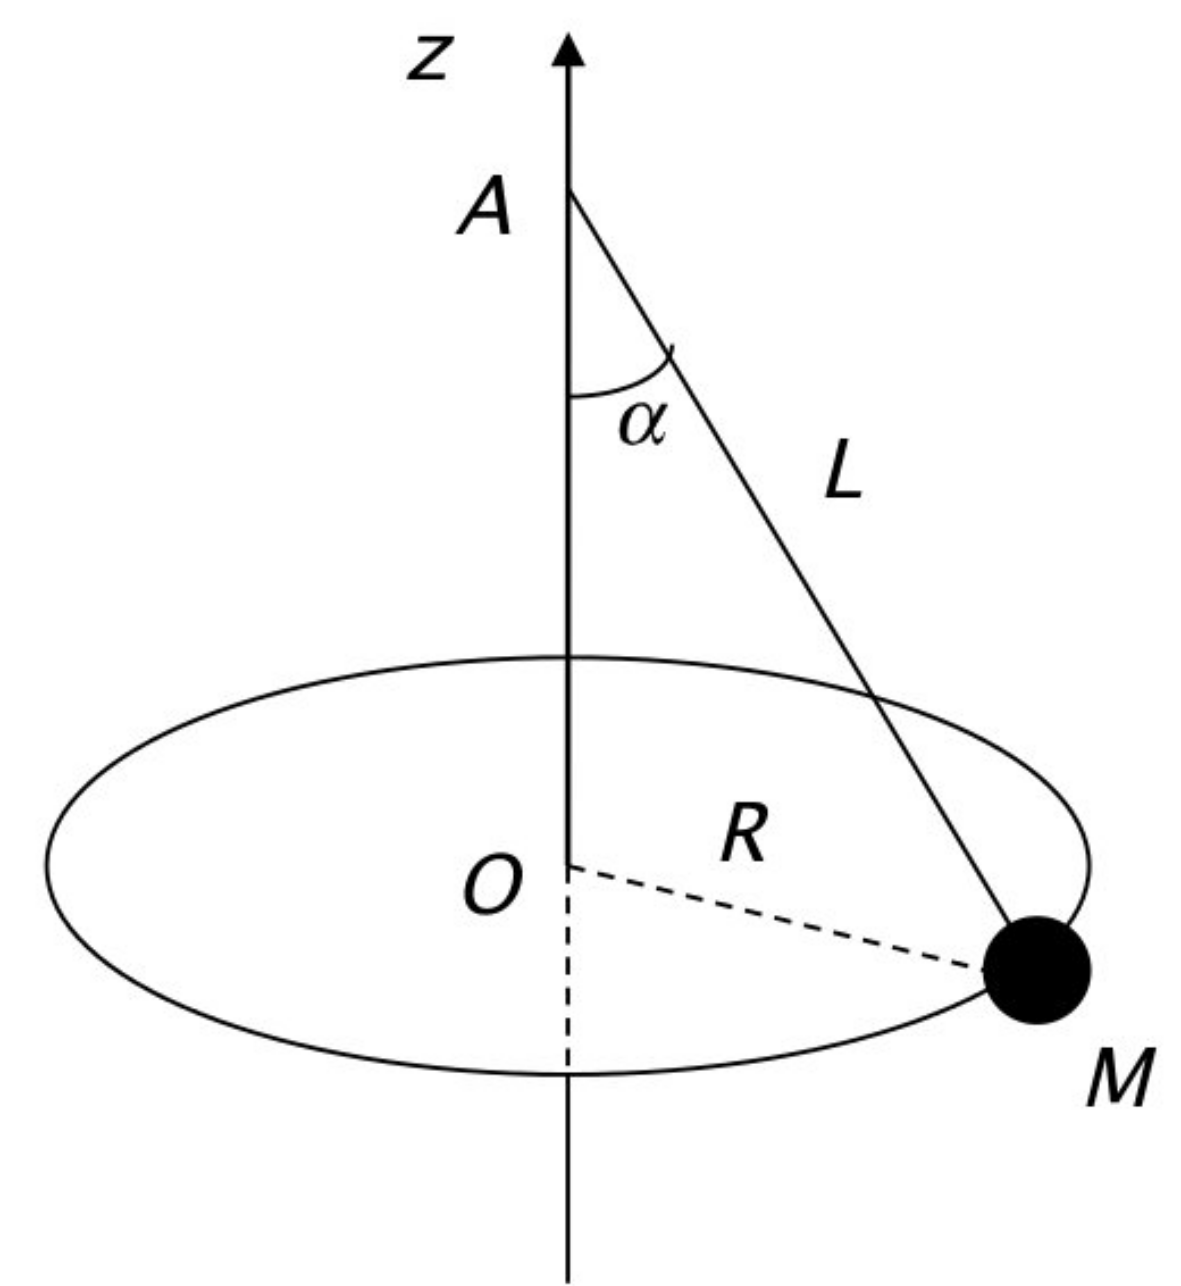
\includegraphics[width=\linewidth]{pendule_conique-plain}
	\end{center}
\end{minipage}

\begin{enumerate}
	\item Exprimer le moment cinétique de M par rapport à A en fonction de $m$,
	      $M$, $\w$ et $\a$.
	\item Appliquer le TMC pour déduire $\cos\a$ en fonction de $g$, $L$ et
	      $\w$.
	\item Retrouver ce résultat à partir du PFD.
\end{enumerate}

\section{Frottements d'un satellite}
% \noindent
% \begin{minipage}[t]{.60\linewidth}
Un satellite S de masse $m$ décrit une trajectoire circulaire uniforme
d'altitude $h_0$ autour de la Terre de masse $m_T$ et de rayon $R_T$, dans le
référentiel géocentrique.
% \end{minipage}
% \hfill
% \begin{minipage}[t]{.30\linewidth}
% 	~
% 	\begin{center}
% 		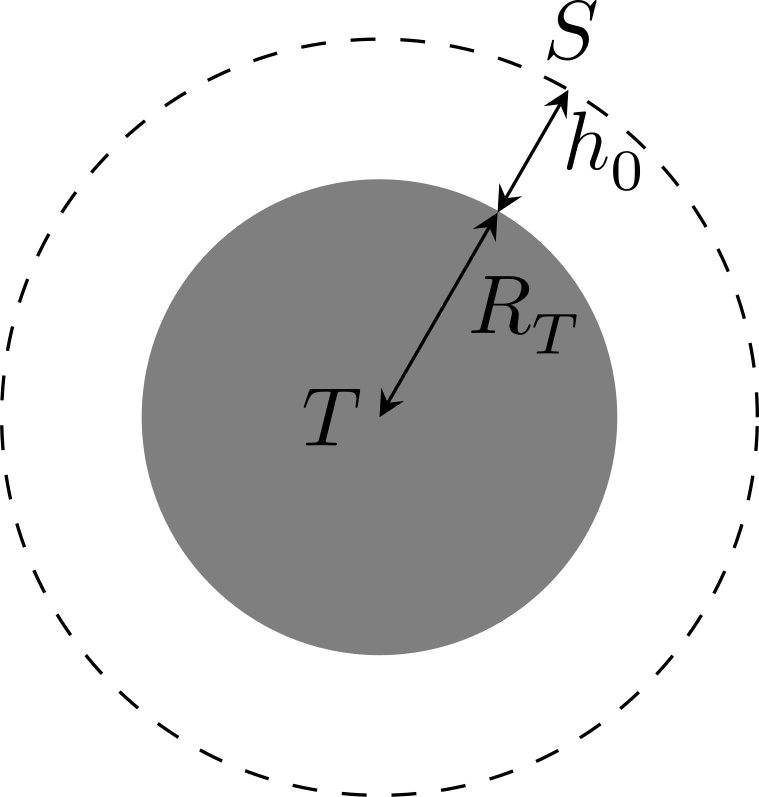
\includegraphics[width=\linewidth]{frott_sat-plain}
% 	\end{center}
% \end{minipage}

\QR{%
	Exprimer la norme $v$ de son vecteur vitesse et son énergie mécanique
	$\Ec_m$ en fonction de $\Gc$, $m_T$, $m$, $R_T$ et $h_0$. On pourra
	localement introduire $R=R_T+h_0$.
}{%
	solu
}

\begin{blocQR}
	\item
	Le satellite étant sur une orbite basse, il subit de la part des
	hautes couches de l'atmosphère une force de frottements qui modifie son
	altitude $h$. Cependant, \textbf{on considère que la trajectoire sur un
		tour reste quasi-circulaire}~; ainsi les expressions précédentes restent
	valables en remplaçant $h_0$ par $h(t)$.
	\QR{%
		Le travail des forces de frottements est-il moteur ou
		résistant~? En déduire le signe de $\dv{\Ec_m}{t}$.
	}{%
		solu
	}

	\QR{%
		Comment évolue le rayon de l'orbite du satellite au cours du
		temps~? Tracer l'allure de sa trajectoire.
	}{%
		solu
	}

	\QR{%
		En déduire le sens de variation de la vitesse. Commenter.
	}{%
		solu
	}

\end{blocQR}

\resetQ
\section{Comète de \textsc{Halley}}

\noindent
\begin{minipage}{0.70\linewidth}
	La comète de \textsc{Halley} est la plus connue. La première mention de son
	observation date de 611 av. J.-C.\ en Chine, et on la retrouve tout au long
	de l'Antiquité et du Moyen Âge, évidemment sans savoir qu'il s'agit d'une
	seule comète. Cette découverte a été formalisée en 1705 par Edmond
	\textsc{Halley,} qui publia un livre avançant que les observations en 1531,
	1607 et 1682 concernaient en fait la même comète. Son prochain passage est
	prévu en 2061. On sait aujourd'hui que la comète de \textsc{Halley} suit une
	trajectoire elliptique de période de révolution autour du Soleil 76 ans, sa
	distance minimale au Soleil étant de $d_{\min} = \SI{0.59}{UA}$.
\end{minipage}
\hfill
\begin{minipage}{.25\linewidth}
	\begin{center}
		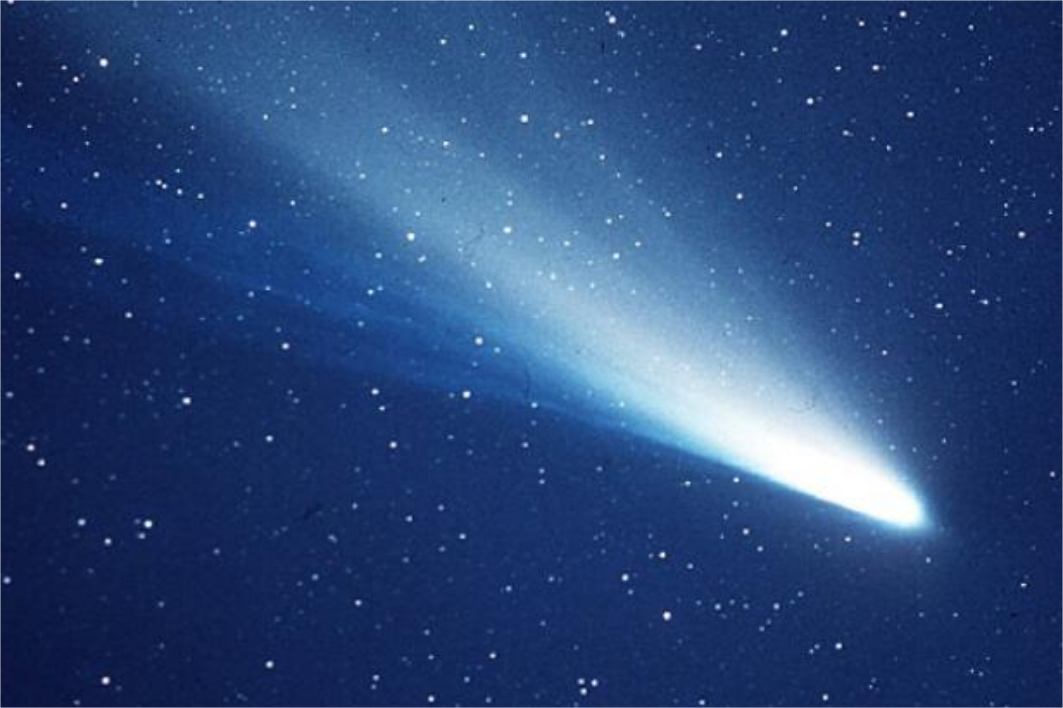
\includegraphics[width=\linewidth]{halley}
	\end{center}
\end{minipage}
\begin{tcb}(defi)<lft>'l'{Données}
	\begin{itemize}
		\item Masse solaire $m_S = \SI{2.0e30}{kg}$.
		\item UA signifie «~unité astronomique~», et correspond à la distance
		      moyenne entre la Terre et le Soleil. $\SI{1}{UA} = \SI{1.5e11}{m}$.
	\end{itemize}
\end{tcb}

\begin{enumerate}
	\item Faire un schéma de la trajectoire de la comète en faisant aussi
	      apparaître la position du Soleil et $d_{\min}$.
	\item Déduire de la troisième loi de \textsc{Kepler} la plus grande distance
	      de la comète au Soleil.
	\item Une conique est décrite par une équation polaire de la forme
	      \[r(\th) = \frac{p}{1-e\cos\th}\]
	      où l'origine du repérage polaire est prise sur un des foyers de la
	      conique. Déterminer le paramètre $p$ et l'excentricité $e$ de la
	      trajectoire de la comète de \textsc{Halley}.
\end{enumerate}

\section{Changement d'orbite}

\noindent
\begin{minipage}{0.70\linewidth}
	Un satellite artificiel assimilé à un point matériel M de masse $m_s$ trouve
	sur une orbite circulaire provisoire de rayon $r_1 = \SI{7500}{km}$ autour
	de la Terre. On souhaite le faire passer sur son orbite définitive de rayon
	$r_2 = \SI{42200}{km}$ (orbite géostationnaire). Pour cela, on le fait
	d'abord passer sur une orbite de transfert elliptique dont le périgée P est
	à la distance $r_1$ et l'apogée A à la distance $r_2$ du centre O de la
	Terre. Dès que le satellite arrive en A, on le fait passer sur l'orbite
	circulaire de rayon $r_2$. Ces deux changements d'orbite sont obtenus par
	allumage d'un moteur placé sur le satellite~: ce processus est très bref
	(par rapport aux périodes orbitales), donc on considérera que la vitesse
	passe instantanément de $v_1$ à $v_{e1}$ en P, puis de $v_{e2}$ à $v_2$ en A
	(sans changer de direction dans les deux cas).
\end{minipage}
\hfill
\begin{minipage}{0.25\linewidth}
	\begin{center}
		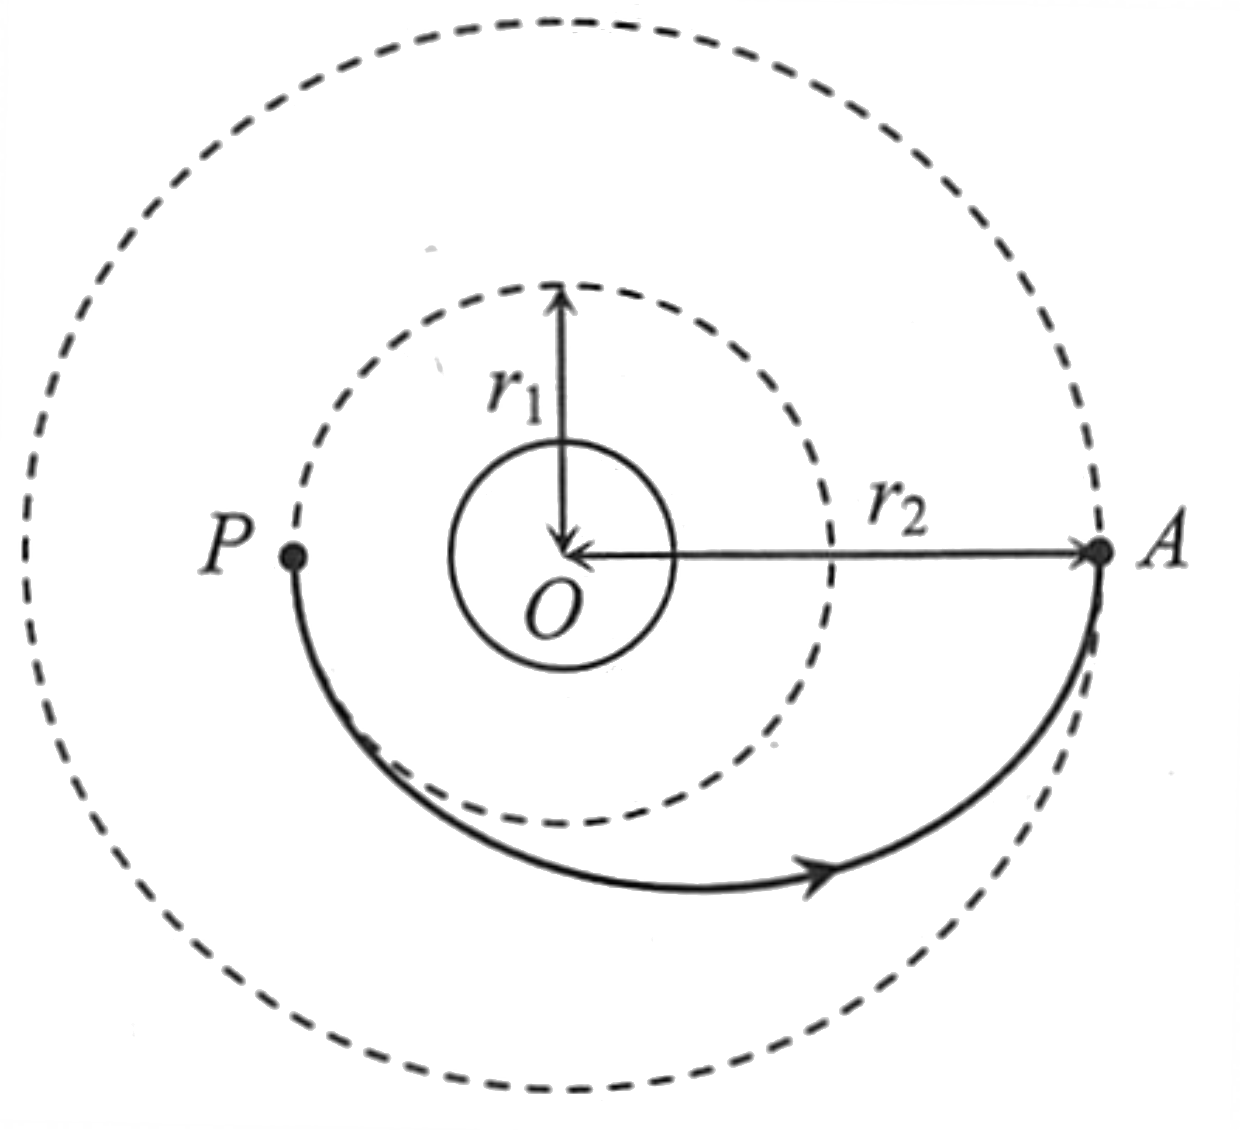
\includegraphics[width=\linewidth]{chgmt_orbite-plain_white}
	\end{center}
\end{minipage}
\begin{tcb}(defi)<lft>'l'{Données}
	$M_{\rm Terre} = \SI{5.97e24}{kg}$~; $\Gc = \SI{6.67e-11}{SI}$.
\end{tcb}

\begin{enumerate}
	\item Calculer la vitesse $v_1$.
	\item Donner l'expression de l'énergie mécanique du satellite sur chacune
	      des trois orbites, en fonction de $r_1$ et $r_2$.
	\item Calculer la vitesse $v_{e1}$ après le premier transfert, et la
	      variation $\D v_P = v_{e1}-v_1$. Calculer également le travail $W_P$
	      fourni par le moteur au satellite en ce point.
	\item Déterminer une relation entre $v_{e1}$, $v_{e2}$, $r_1$ et $r_2$.
	      Calculer $v_{e2}$.
	\item Calculer la variation de vitesse $\D v_A = v_2 - v_{e2}$ lors du
	      second transfert, ainsi que le travail $W_A$ fourni par le moteur au
	      satellite.
\end{enumerate}

% TODO: Ajouter énoncés suivants~:

% Alerte à l'astéroïde
% Modèle de Bohr
% Expérience de Rutherford

\resetQ
\section{Alerte à l'astéroïde~!}
\noindent
\begin{minipage}[c]{.45\linewidth}
	~
	\begin{center}
		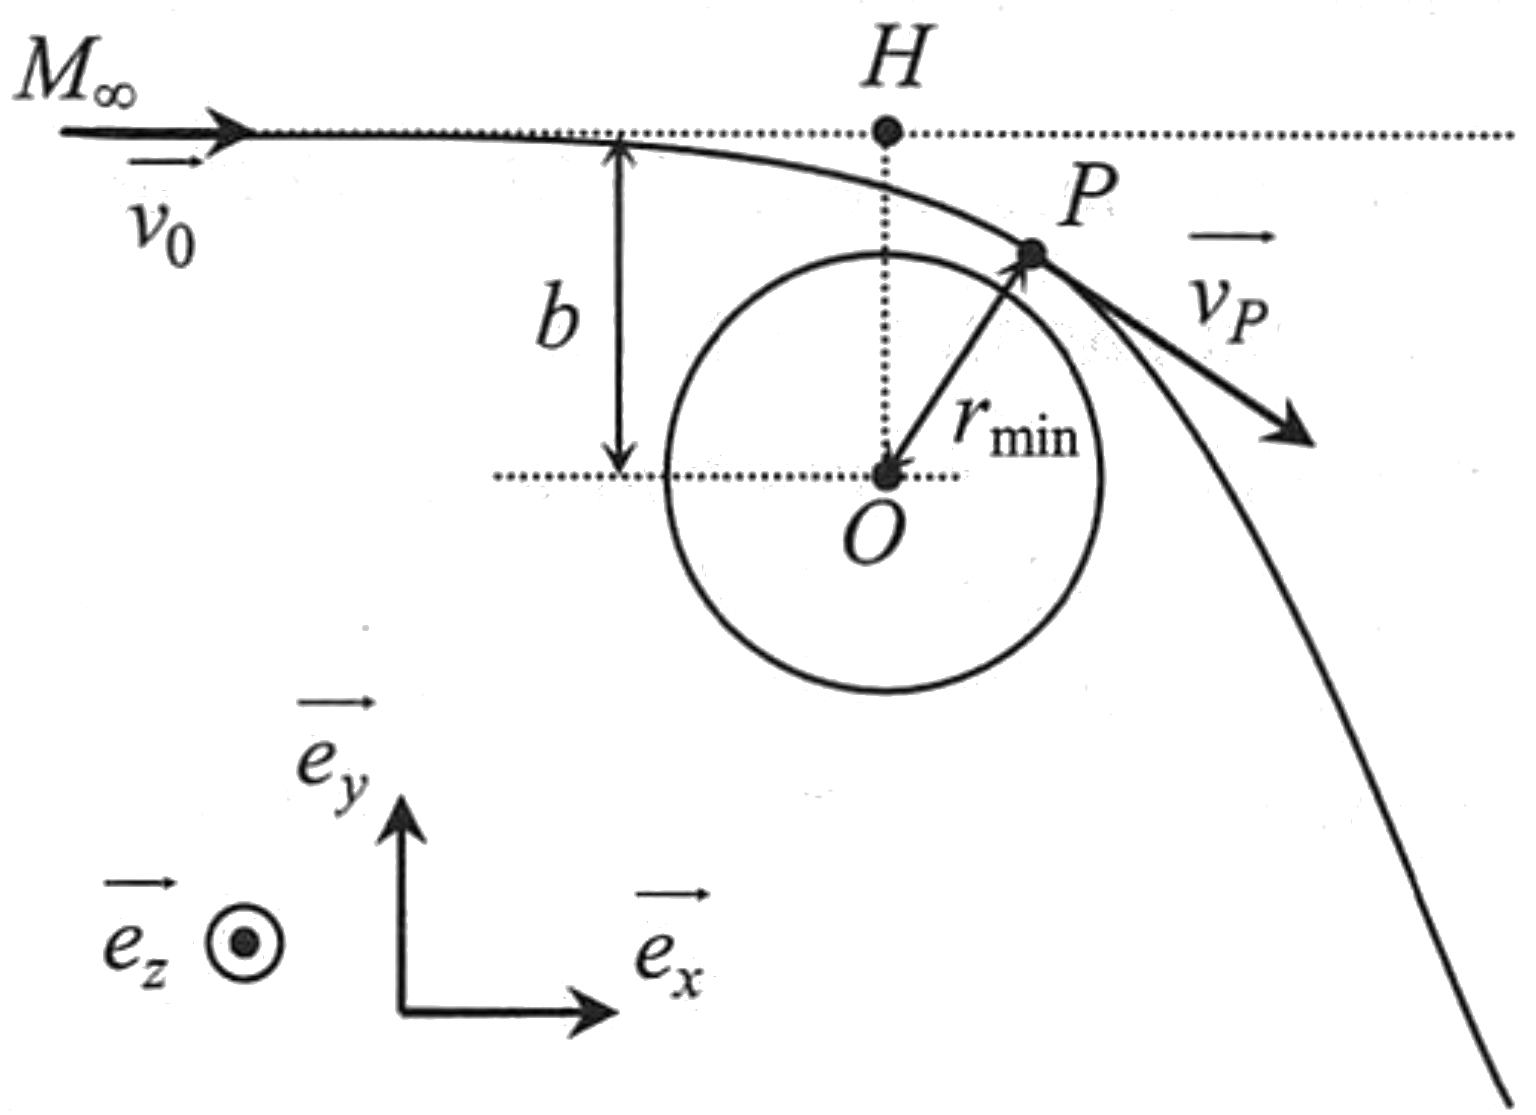
\includegraphics[width=\linewidth]{alerte_aste-plain_white}
		\captionof{figure}{Trajectoire de l'astéroïde.}
		\label{fig:aste}
	\end{center}
\end{minipage}
\hfill
\begin{minipage}[c]{.50\linewidth}
	De nombreux objets, dits géocroiseurs, passent à proximité de la Terre… et
	parfois la heurtent~!
	\smallbreak
	On considère ici un astéroïde de masse $m$ actuellement très éloigné de la
	Terre et de tout autre astre. Il a donc un vecteur vitesse $\vfo$ constant. Le
	prolongement de sa trajectoire rectiligne passe à une distance $b$ (appelée
	paramètre d'impact) du centre O de la Terre.
	\smallbreak
	Cependant lorsqu'il se rapprochera de la Terre, l'attraction gravitationnelle
	de celle-ci va dévier l'astéroïde selon une trajectoire hyperbolique. On
	appelle périgée le point P de cette trajectoire le point le plus proche du
	centre de la Terre.
\end{minipage}

\QR{%
	Quelles sont les deux grandeurs dynamiques de l'astéroïde qui se consservent
	au cours de son mouvement~? Traduire en équation leurs conservations entre les
	deux position $\Mr_{\infty}$ et P.
}{%
	solu
}
\QR{%
En déduire la distance minimale d'approche $r\ind{min} = {\rm OP}$.
}{%
solu
}
\QR{%
	Application numérique~: $v_0 = \SI{2.0}{km.s^{-1}}$ et $b = \SI{140000}{km}$.
	L'astéroïde va-t-il heurter la Terre~?
}{%
	solu
}

\resetQ
\section{Modèle de \textsc{Bohr} de l'atome d'hydrogène}
Pour expliquer le spectre de raies de l'atome d'hydrogène observées
expérimentalement, Niels Bohr a proposé un modèle qui s'appuie sur les
hypothèses suivantes~: dans un référentiel galiléen lié au noyau O,
\smallbreak
\noindent
\begin{minipage}[t]{.68\linewidth}
	\begin{itemize}
		\item L'électron décrit une trajectoire circulaire sur laquelle il ne
		      rayonne pas d'énergie~;
		\item l'électron échange de l'énergie avec l'extérieur sous forme de lumière
		      lorsqu'il change de trajectoire circulaire~;
		\item la norme du moment cinétique de l'électron est quantifié et ne peut
		      prendre que des valeurs discrètes vérigiant la relation~:
		      \[
			      \Lc_{O_n} = n \times \frac{h}{2\pi}
			      \quad
			      n \in \Nb^{*}
		      \]
		      avec $h = \SI{6.63e-34}{J.s}$
	\end{itemize}
\end{minipage}
\hfill
\begin{minipage}[t]{.30\linewidth}
	~
	\begin{center}
		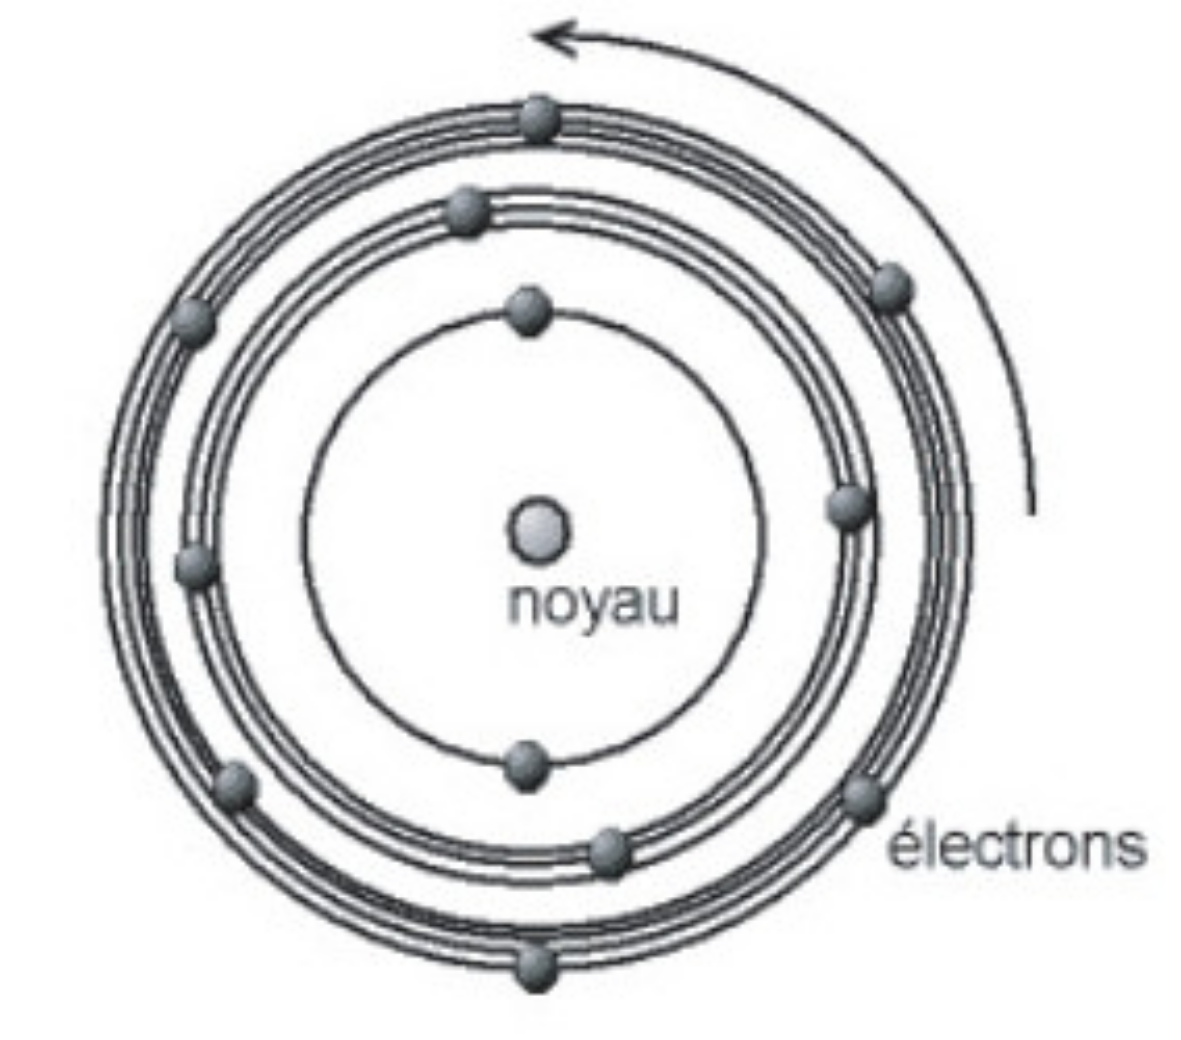
\includegraphics[width=\linewidth]{mod_bohr-plain}
	\end{center}
\end{minipage}

\smallbreak
Une orbitale électronique correspond à une valeur de l'entire $n$. Elle est
caractérisée par un rayon $r_n$, une vitesse $v_n$ et une énergie mécanique
$\Ec_{m}(n)$.
\smallbreak
Ce modèle semi-classique n'est pas complètement satisfaisant, mais il prédit
le spectre de raies de l'atome d'hydrogène.
On rappelle qu'un atome d'hydrogène est consitué d'un oyau (charge $e =
	\SI{1.602e-19}{C}$, masse $m_p$) et d'un électron (charge $-e$, masse $m_e =
	\SI{9.11e-31}{kg}$). On donne les valeurs numériques de la célérité de la
lumière dans le vide $c = \SI{3.00e8}{m.s^{-1}}$ et la permittivité
diélectrique du vide $\ep_0 = \SI{8.85e-12}{F.m^{-1}}$.
\QR{%
	Rappele l'expression de la force d'interaction exercée par le noyau sur
	l'électron et de l'énergie potentielle dont elle dérive.
}{%
	solu
}
\QR{%
Utiliser le fait que les orbitales soient circulaires pour exprimer le carré
$v_n{}^{2}$ de la vitesse de l'électron en fonction de la distance $r_n$.
}{%
solu
}
\QR{%
	Utiliser la quantification du moment cinétique pour exprimer le rayon de la
	trajectoire en fonction de $n$, $h$, $m_e$ et $e$.
}{%
	solu
}
\QR{%
	Calculer sa valeur pour $n=1$.
}{%
	solu
}
\QR{%
	Exprimer l'énergie mécanique $\Ec_m(n)$ de l'électron et montrer qu'elle se
	met sous la forme $\Ec_m(n) = -\frac{A}{n^2}$. Donner l'expression et la
	valeur numérique de $A$ en électron-volts (on rappelle que $\SI{1}{eV} =
		\SI{1.6e-19}{J}$).
}{%
	solu
}
\QR{%
	Sachant que le passage d'un niveau d'énergie $\Ec_m(n_2)$ à un autre
	$\Ec_m(n_1)$ se traduit par l'émission d'un pgoton de fréquence $\nu$ telle
	que $\Delta{E} = h\nu$, en déduire que les longueurs d'onde $\lambda$ émises
	vérifient~:
	\[
		\frac{1}{\lambda} =
		R_H \left( \frac{1}{n_2{}^{2}} - \frac{1}{n_1{}^{2}} \right)
	\]
	On rappelle que $\nu = c/\lambda$. On donnera l'expression de la constante
	de \textsc{Rydberg} $R_H$ et sa valeur numérique.
}{%
	solu
}

\resetQ
\section{Expérience de \textsc{Rutherford}}
Entre 1909 et 1911, Ernest \textsc{Rutherford} et ses deux étudiants Hans
\textsc{Geiger} et Ernest \textsc{Marsden} ont réalisé et interprété une
expérience consistant à bombarder une mince feuille d'or avec des particules
$\alpha$ (que \textsc{Rutherford} avait précédemment identifiées comme des
noyaux d'hélium). Ils observèrent que la plupart de ces particules
traversaient la feuille sans être affectées (donc ne rencontraient que du
vide), mais que certaines étaient déviées, parfois très fortement~: les angles
de déviation pouvant être reliés aux dimensions microscopiques, cela permi la
découverte du noyau atomique et l'estimation de sa taille.
\smallbreak
\noindent
\begin{minipage}[c]{.48\linewidth}
	On considère ici une particule $\alpha$ de masse $m$ et de charge $+2e$, venant
	de l'infini avec la vitesse $\vfo = v_0\ex$, et s'approchant avec le paramètre
	d'impact $b$ d'un noyau cible de numéro atomique $Z$. La particule est repérée
	par ses coordonnées polaires $(r,\th)$ dans le plan $(\Or xy)$.
	\bigbreak
	Le noyau reste pratiquement immobile dans le référentiel terrestre~: on
	travaille dans ce référentiel supposé galiléen, le repère étant centré sur la
	position O du noyau. La trajectoire suivie par la particule $\alpha$ est une
	branche d'hyperbole représentée ci-contre.
\end{minipage}
\hfill
\begin{minipage}[c]{.48\linewidth}
	\begin{center}
		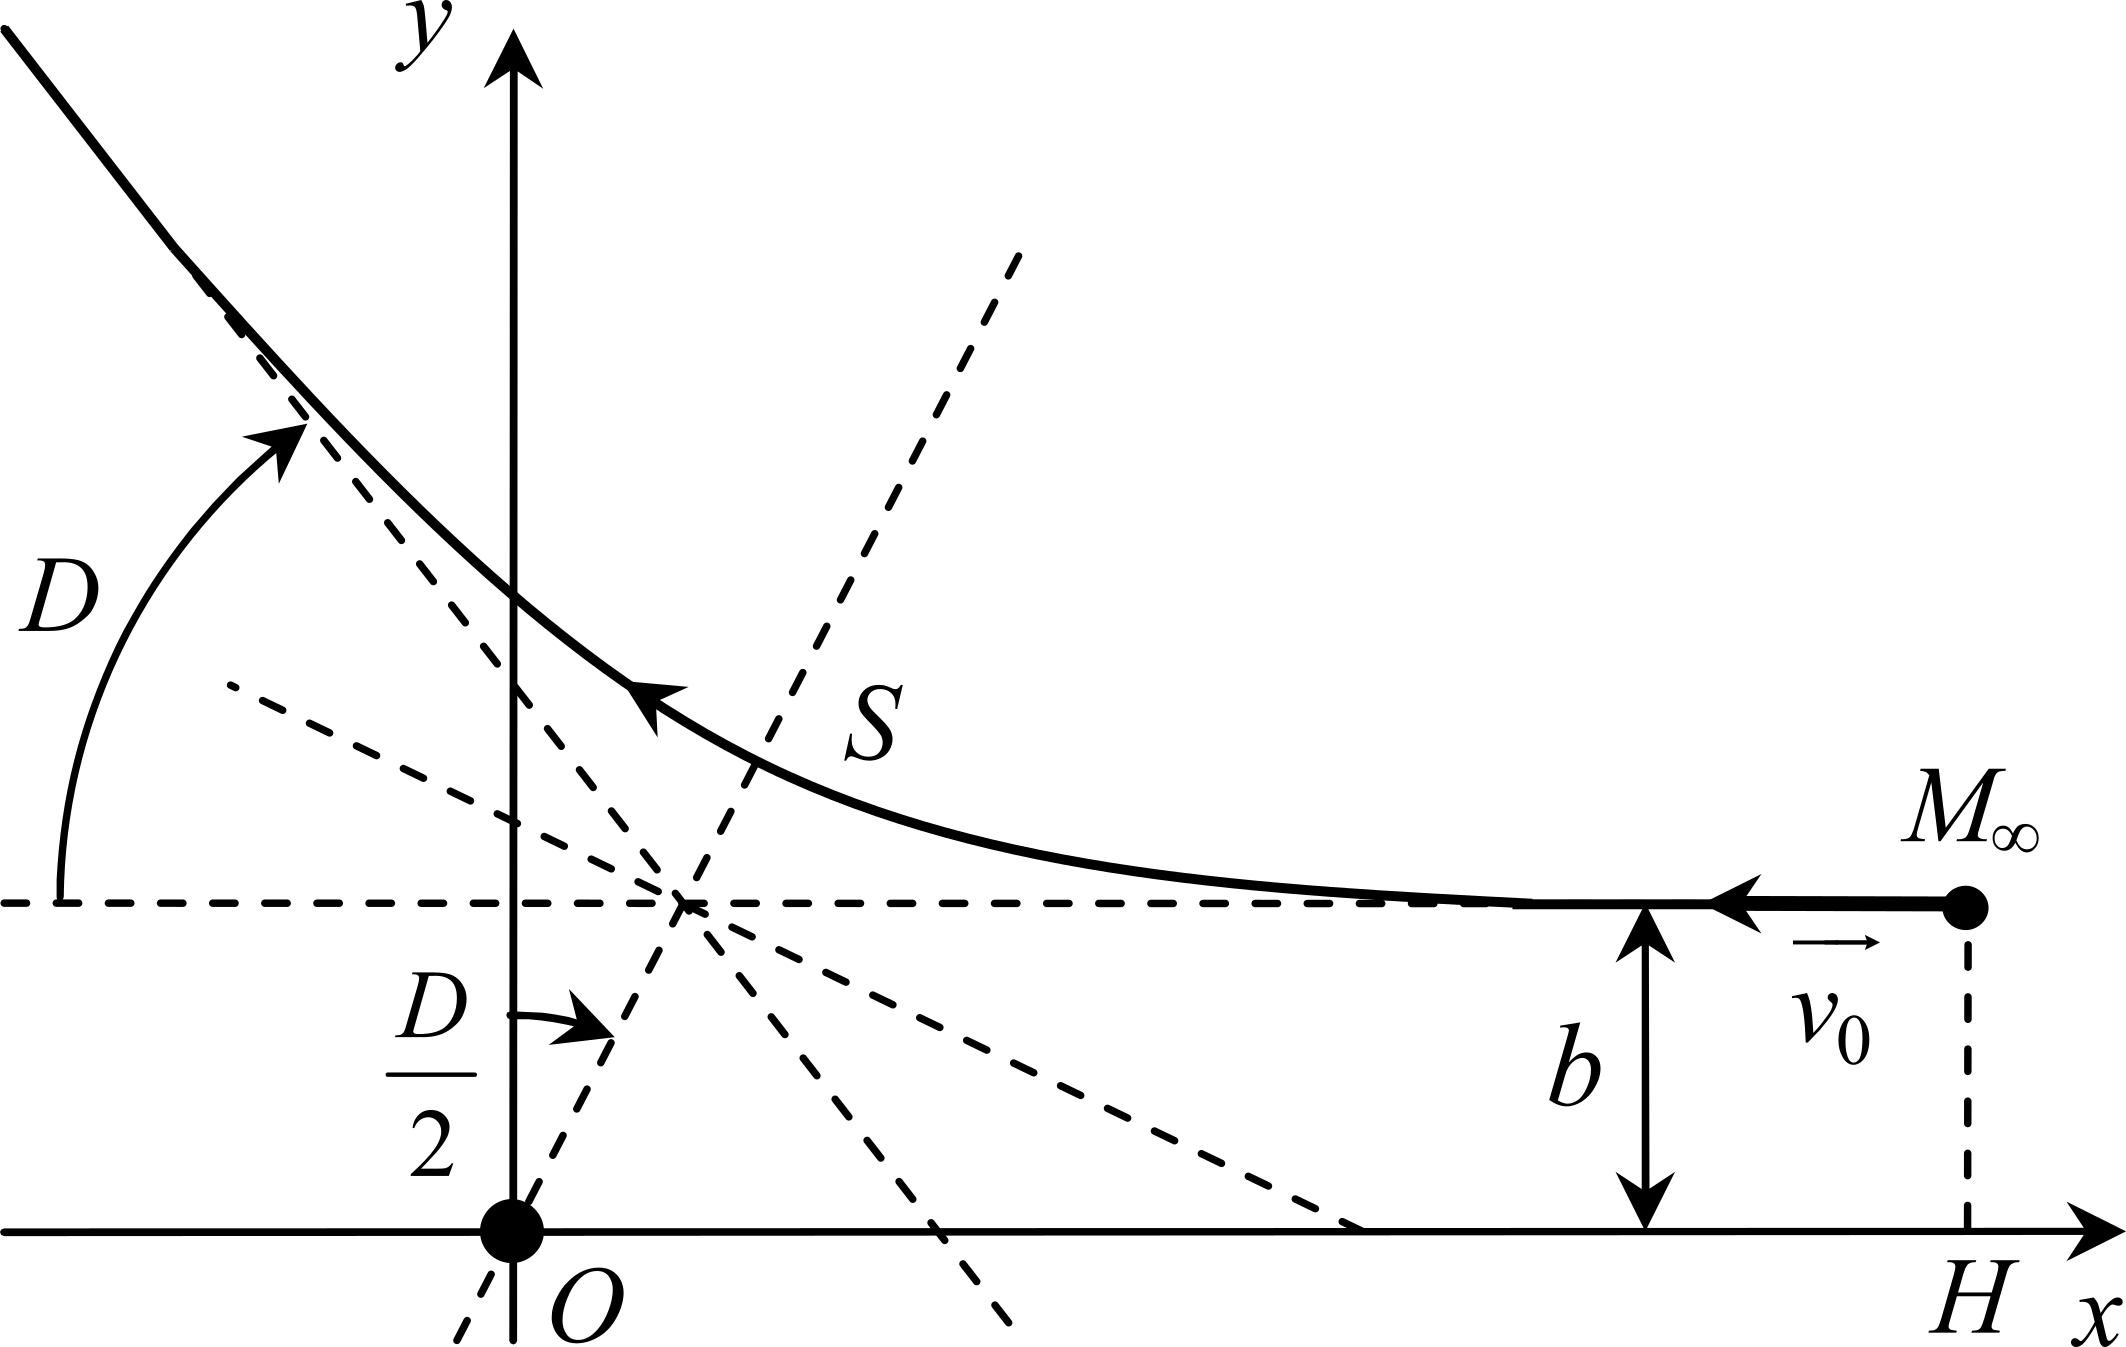
\includegraphics[width=\linewidth]{ruth-plain}
		\captionof{figure}{Trajectoire suivie par la particule $\alpha$.}
		\label{fig:ruth}
	\end{center}
\end{minipage}

% \begin{figure}[htbp]
% 	\centering
% 	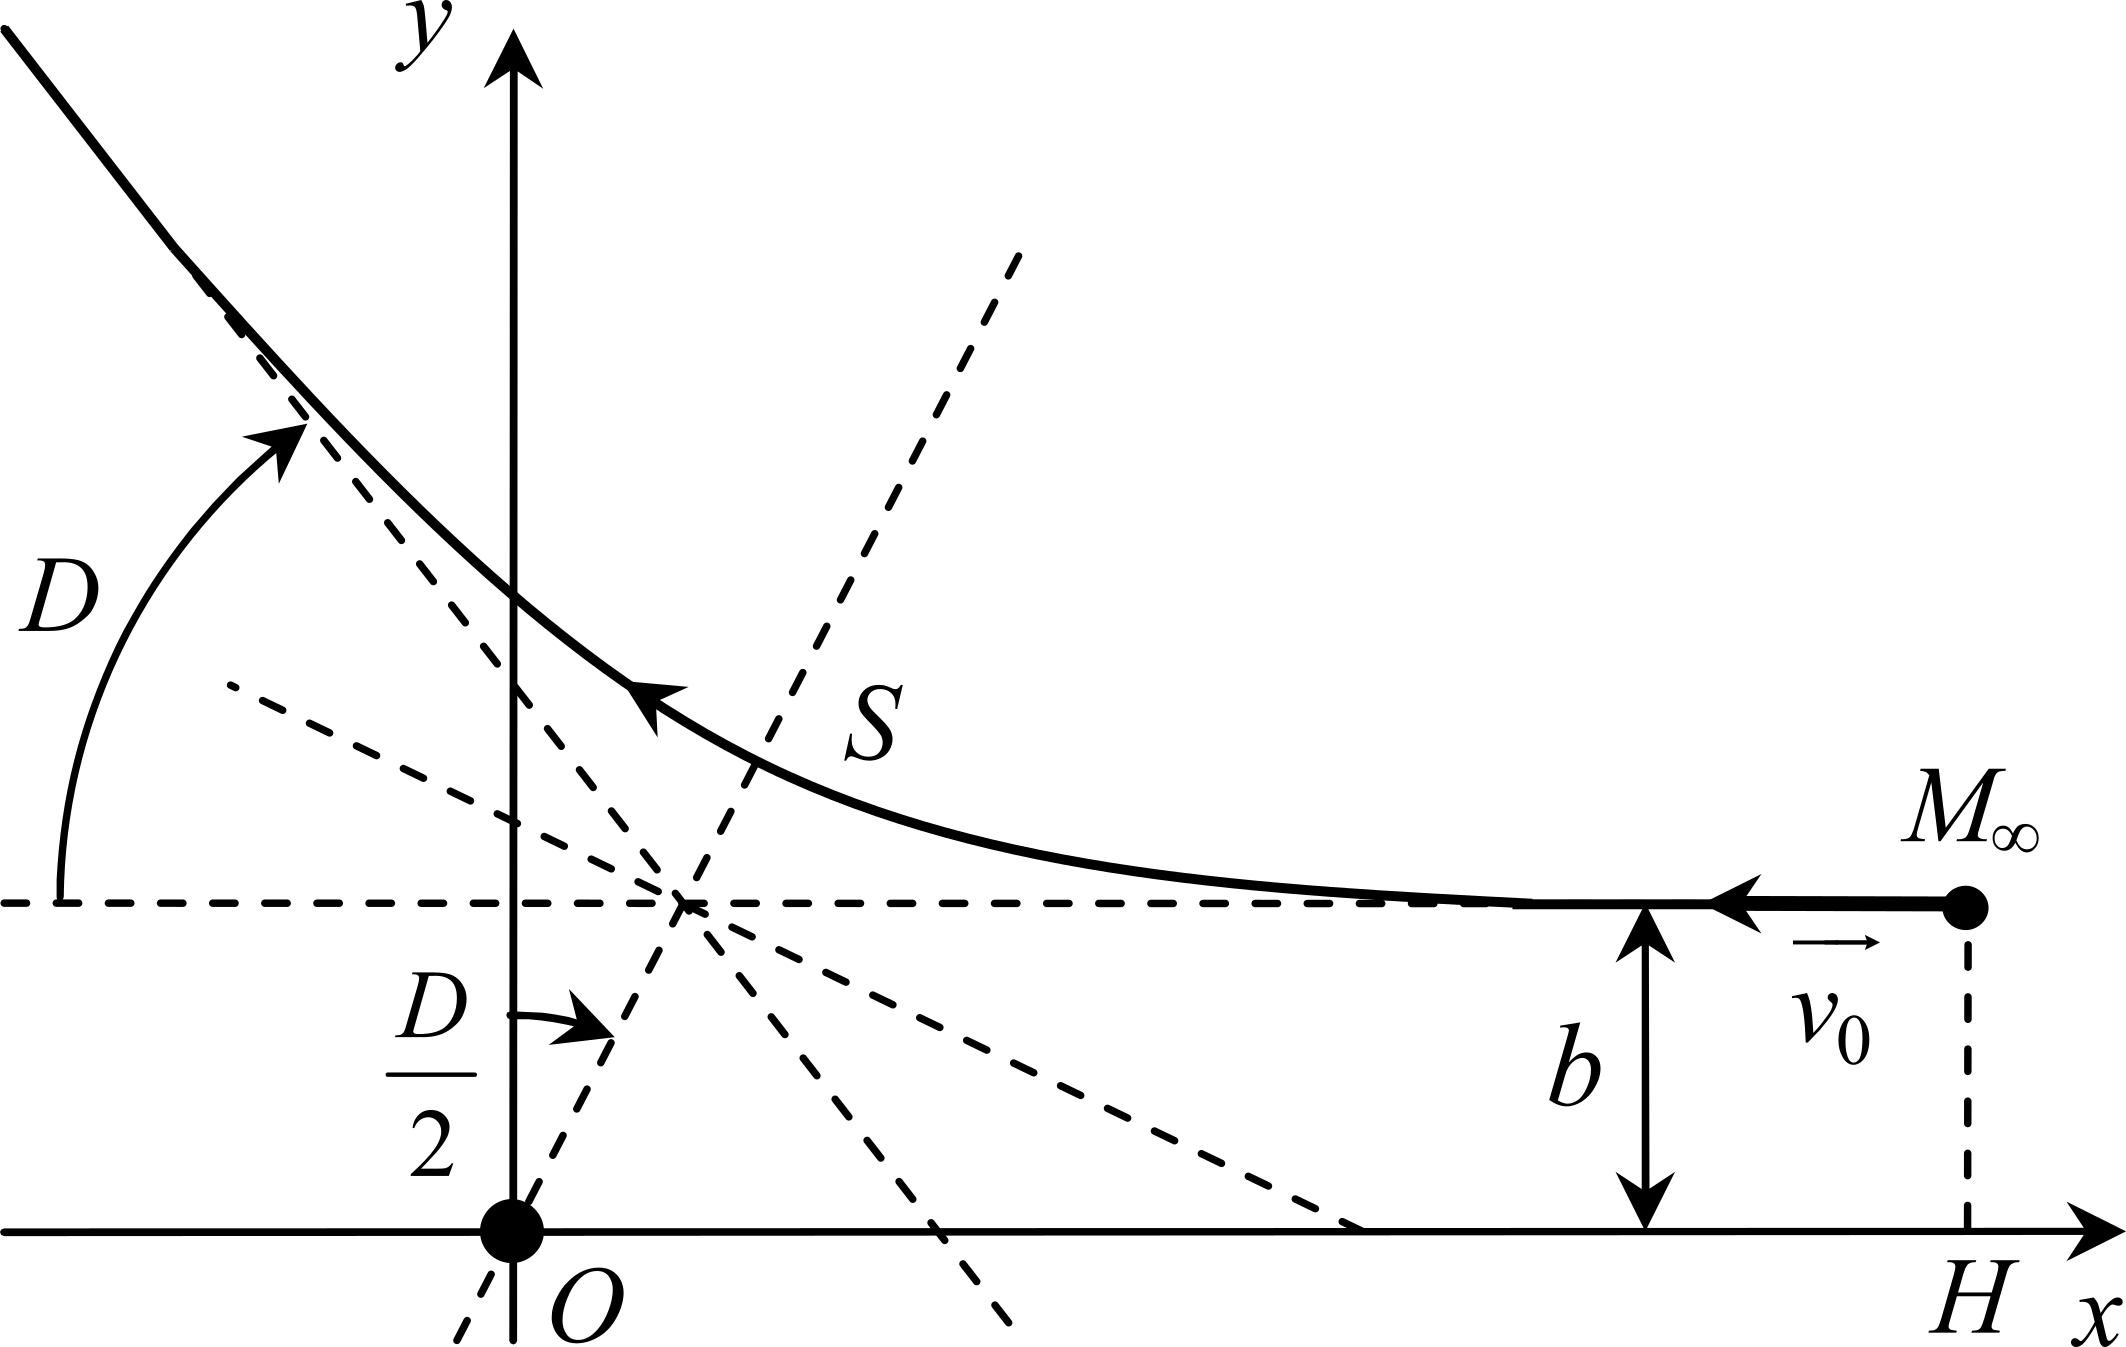
\includegraphics[width=.6\linewidth]{ruth-plain}
% 	\caption{Trajectoire suivie par la particule $\alpha$.}
% 	\label{fig:ruth}
% \end{figure}
\QR{%
	Donner l'expression de la force électrique subie par la particule $\alpha$,
	sous la forme $\Ff = \frac{K}{r^{2}}\er$ ainsi que celle de son énergie
	potentielle d'interaction.
}{%
	solu
}
\QR{%
	Montrer que l'énergie mécanique $\Ec_m$ de la particule $\alpha$ est une
	constante du mouvement et donner sa valeur.
}{%
	solu
}
\QR{%
	Montrer que le moment cinétique $\Lcf_{\Or}$ de la particule $\alpha$ en O est
	un vecteur constant, et donner la valeur de cette constante à l'aide des
	conditions initiales. Montrer que $\Lcf_{\Or}$ s'exprime de manière simple en
	fonction des variables $r$ et $\tp$.
}{%
	solu
}
\QR{%
	Montrer que l'énergie mécanique peut se mttre sous la forme $\Ec_m =
		\frac{1}{2}m \rp^{2} + \Ec_p'(r)$ et expliciter la fonction $\Ec_p'(r)$.
	Comment l'appelle-t-on~?
}{%
	solu
}
\QR{%
On note S la position de la particule $\alpha$ pour laquelle elle passe au
plus près du noyau d'or, et on note $r_{\min} = \rm OS$ la distance minimale
d'approche. Que revient l'expression de $\Ec_m$ lorsque $r = r_{\min}$~? En
déduire que
\[
	r_{\min} = \frac{K}{mv_0{}^{2}}
	\pac{1 + \sqrt{1 + \left( \frac{mbv_0{}^{2}}{K} \right)^{2}}}
\]
}{%
solu
}
\QR{%
On donne $\ep_0 = \SI{8.9e-12}{F.m^{-1}}$, $e = \SI{1.6e-19}{C}$, $m =
	\SI{6.6e-27}{kg}$, $v_0 = \SI{2.0e7}{m.s^{-1}}$ et $Z = 79$ pour l'or. D'autre
part, on peut montrer que l'angle de déviation $D$ de la particule est donné
par la relation
\[
	\tan(\frac{D}{2}) = \frac{K}{mbv_0{}^{2}}
\]
Calculer $b$ puis $r_{\min}$ pour $D_1 = \ang{60}$ et pour $D_2 = \ang{180}$
(particule envoyée vers l'arrière). En déduire l'ordre de grandeur de la
taille du noyau d'or.
}{%
solu
}

\end{document}
